
In this project you will implement a phrase-based translation system.
You will experiment with monotone translation and lattice translation.
Importantly, you will learn about formal tools such as finite-state transducers and the underlying complexity of the translation problem.

In summary, you will experiment with

\begin{itemize}
	\item monotone translation
	\item decision rules
	\item preordering and lattice translation
\end{itemize}

You will not implement finite-state transducers (and their operations) yourselves, instead you are expected to use \texttt{OpenFST} \citep{Allauzen+2007:OpenFST}.\footnote{\url{http://www.openfst.org}}
We advise you to use the command line tools provided with the library for they are {\bf much simpler to use} than the \texttt{C++} API.
The illustrations in this document were all produced by \texttt{OpenFST} and that is what you should use in your report.
There is a tutorial on design and operations\footnote{\url{http://www.openfst.org/twiki/bin/view/FST/FstHltTutorial}} and another on applications\footnote{\url{http://www.openfst.org/twiki/bin/view/FST/FstSltTutorial}}.
For a very comprehensive survey on weighted automata algorithms refer to \citep{Mohri:2009:WAA}. 

We are providing data for a development set of English-Japanese sentence pairs.\footnote{\url{https://wilkeraziz.github.io/uva-nlp2/resources/project2/data/pbsmt.tgz}} The data amounts to 1416 sentence pairs, and even though you may experiment with as many sentences as you like, you are expected to submit results only for the first 100 sentence pairs. 
The data folder contains \textsc{Readme} files with additional information, but in sum you will find:
\begin{itemize}
	\item Source, reference and permutations
	\item Phrase tables
	\item Examples of packed permutations
	\item Examples of translations
	\item Model parameters
\end{itemize}



\section{Phrase-based MT}


In phrase-based MT \citep{Koehn+2003:pbsmt}, we do not have a proper generative model from where we can infer latent derivations and thus generate translations of an input sentence.
Instead, we create a large repository of rules (phrase pairs) from some large word-aligned training data.
Rules consist of phrase pairs extracted by enumeration of connected subsets of word alignments -- check \citep{Koehn+2003:pbsmt} for a more precise definition.
Then, for a given input, we instantiate the space of possible translations by concatenating known phrase pairs in target word order such that they cover some permutation of the input sentence.\footnote{This is reminiscent of data-oriented parsing \citep{Bod:1992:DOP}.}
To keep the solution tractable, we impose some form of limit to reordering (typically by means of a distortion limit).
Once the space of translations is defined, we score each and every hypothesis using a linear model.
Because the features of this linear model are rather local (e.g. at the level of phrases or short target $n$-grams), this scoring can be done quite efficiently in a packed representation of the complete set of translation derivations (that is, there is no need for enumeration as in a list).
In this project, you will assume the parameters of the linear model are known, and you will explicitly instantiate the weighted set of translation derivations of a given input.
You will also experiment with different decision rules, i.e., ways in which to select one translation as output.\footnote{In project 3, you will fit the parameters of the linear model to data using discriminative learning algorithms.}

\section{Tasks}

You will implement phrase-based MT using finite-state transducers. 
Some of the constructs are similar to those presented by \citet{Knight+1998:WBFST} for word-based models based on IBM$_{\ge 3}$ and by \citet{Kumar+2003:WFST} for the alignment template model.
For example, check Figure 1 in \citep{Kumar+2003:WFST} for a general architecture. 
Keep in mind that phrase-based MT does not offer explicit models for segmentation and permutation. Segmentation is basically guided by the known source phrases and permutation is arbitrary within a distortion limit. 
A few features are designed in an attempt to capture segmentation and permutation preferences, such as phrase-penalty and distortion cost.



\subsection{Task 1: source sentence}

A source sentence can be seen as a trivial linear finite-state acceptor whose arcs are labelled with the words in original order. Consider the example \texttt{the black dog}, Figure \ref{fig:src} illustrates one way to encode it as a transducer.\footnote{Obviously, there are different ways to do so. I chose to encode it as a transducer from 0-based input positions to source words because the positions will turn out to be useful when we are interested in retrieving the alignment between source and target after translation.}

\begin{figure}[h]\centering
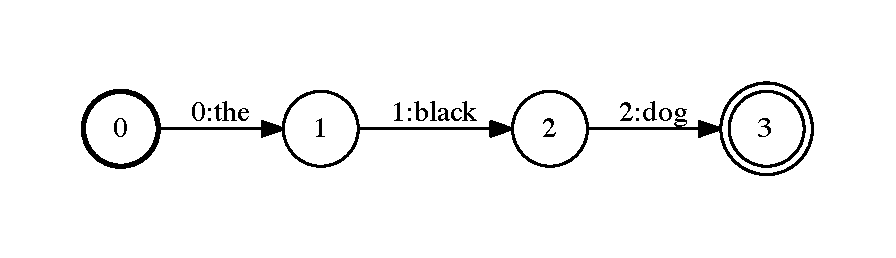
\includegraphics[scale=0.5]{src.pdf}
\caption{\label{fig:src}Input seen as a transducer: the label encodes an input position and its corresponding word.}
\end{figure}

Table \ref{tab:task1} summarises the task. 

\begin{table}[h]\centering
\begin{tabular}{l p{12cm}}
\textsc{Task}   &  encode source sentences as transducers \\
\textsc{Input}  &  first 100 English sentences in \texttt{dev.en} \\
\textsc{Output} &  one transducers for each sentence\\
\textsc{Submit} & nothing to submit here\\
\textsc{Report} & add a graphical illustration for one example from \texttt{dev.en} \\
\end{tabular}
\caption{\label{tab:task1}Task 1 summarised}
\end{table}

\subsection{Task 2: phrase table}


A phrase-table can be seen as recursive finite-state transducer that maps contiguous sequences of source words onto contiguous sequences of target words. 
Consider the rules in Figure \ref{fig:table}, Figure \ref{fig:rules} shows the resulting transducer: its initial state is also final, other states are introduced in order to memorise phrase pairs (we first read a source phrase outputting empty strings, then we produce a target phrase consuming empty strings).
Note that the phrase table transducer defines an infinite set of binary relations over $\Sigma^* \times \Delta^*$ (where $\Sigma$ is the source language vocabulary and $\Delta$ is the target language vocabulary).


\begin{figure}[h]\centering
\begin{tabular}{l l }
\bf Source & \bf Target \\
\texttt{the} & \texttt{le}  \\
\texttt{the} & \texttt{un} \\
\texttt{dog} & \texttt{chien} \\
\texttt{black} & \texttt{noir} \\
\texttt{black} & \texttt{noirs} \\
\texttt{black dog} & \texttt{chien noir} 
\end{tabular}
\caption{\label{fig:table}Example phrase table.}
\end{figure}


In this task you will have to produce a weighted finite-state transducer for each of the first 100 sentences in \texttt{dev.en}. 
Under \texttt{rules.monotone.dev} you will find one phrase table for each source sentence, they are stored in files named \texttt{grammar.$n$} where \texttt{$n$} is the sequential (0-based) position of the sentence in \texttt{dev.en}.


\begin{figure}[h]\centering
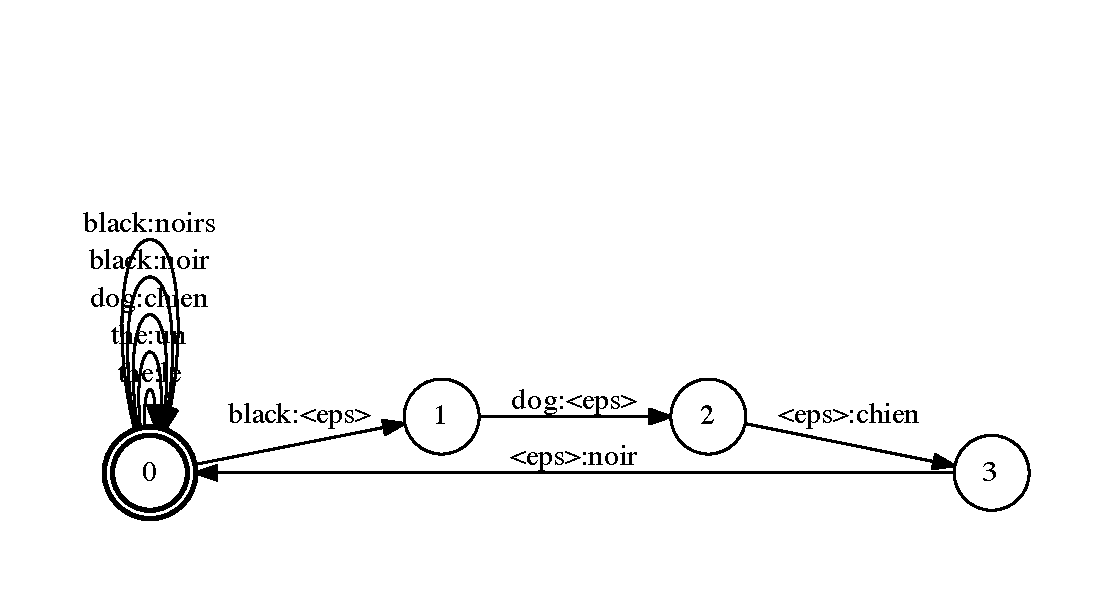
\includegraphics[scale=0.5]{table.pdf}
\caption{\label{fig:rules}Phrase table as a transducer.}
\end{figure}

In a grammar file, each rule is represented by 5 fields separated by 3 vertical bars:

\begin{itemize}
	\item the first field can be ignored
	\item the second field contains the source phrase
	\item the third field contains the target phrase
	\item the fourth field contains a feature map:
		\begin{itemize}
			\item \texttt{IsSingletonF}: whether the source phrase occurred only once in the training data
			\item \texttt{IsSingletonFE}: whether the phrase pair occurred only once in the training data
			\item \texttt{SampleCountF}: frequency of the source phrase in the training data 
			\item \texttt{CountEF}: frequency of the phrase pair in the training data 
			\item \texttt{EgivenFCoherent}: frequency of the target phrase normalised w.r.t. frequency of source phrase
			\item \texttt{MaxLexEgivenF}: lexical smoothing
		\end{itemize}
	\item the last field (which you can ignore) represents the internal alignment of the phrase pair
\end{itemize}

In a phrase-based system, translation rules are parametrised by a linear model.
Let $(f, e)$ be a phrase pair and $\phi: \Sigma^+ \times \Delta^+ \to$ a mapping between phrase pairs and a $d$-dimensional feature vector.
Then each phrase pair $(f,e)$ is associated with a parameter $\theta_{(f,e)} = w^\top \phi(f,e)$ where $w$ is a vector of model parameters.
You will note that rules are annotated with features, those are components in the linear model. You will need those, and the model parameters in \texttt{weights.monotone}, in order to score phrase pairs. 
Besides the features in the phrase table, you need to consider 3 other features which also decompose at the phrase level, but aim mostly at scoring segmentations, namely:
\begin{itemize}
	\item \texttt{Glue}: the total number of phrases used in a derivation - each phrase pair contributes to this feature with a count of $1$
	\item \texttt{WordPenalty}: the total number of target words in a derivation - each phrase pair contributes to this feature with $\frac{-1}{\ln(10)}$ times the number of tokens in the target phrase 
%	\item \texttt{PassThrough}: typically, each unknown source word (a word without an entry in the phrase table) motivates a ``pass-through'' rule, that is, a trivial phrase pair that copies that unknown source word onto the output stream - each such rule contributes to this feature with a count of $1$
\end{itemize}

Finally, to make sure phrase tables can cover all words in the input we typically augment them with ``passthrough rules'' (attention: the phrase tables we provide do not contain such rules, you have to take care of that yourself).
A passthrough rule is a trivial rule that copies a symbol from the input stream onto the output stream. 
%Another way to translate source words which are unknown to the phrase table is to replace them with a special symbol, such as \texttt{Unk}, and add a transition that translates this symbol to itself.
%Whatever strategy you choose, make sure you account for the \texttt{PassThrough} feature when computing the weight of each phrase pair. 
If you watch carefully, you will see that we provided a model parameter for the feature \texttt{PassThrough}.
This feature simply counts the number of passthrough rules used in a derivation, in other words, it captures how many source words were unknown. 
Note that as defined, each ``passthrough phrase pair'' contributes to this feature with a count of $1$.
In most cases, this feature is meaningless as the number of unknown source words is constant for each source sentence. 
In practice, for reasons beyond the scope of this section, translation systems might estimate a parameter for this features nevertheless.

Table \ref{tab:task2} summarises the task. 

\begin{table}[h]\centering
\begin{tabular}{l p{12cm}}
\textsc{Task}   &  encode phrase tables as transducers \\
\textsc{Input}  &  one phrase table per English sentence: \texttt{rules.en-ja.dev.tgz} \\
\textsc{Output} &  one transducers per phrase table in \texttt{rules.en-ja.dev.tgz} \\
\textsc{Submit} &  nothing to submit here\\
\textsc{Report} & discuss the steps involved in creating a phrase table transducer and scoring its arcs, illustrate fragments of phrase tables containing at least one phrase of each of the following types: $1-1$, $m-n$ with $n > m$ and with $m > n$\\
\end{tabular}
\caption{\label{tab:task2}Task 2 summarised}
\end{table}


\section{Monotone word replacement models}

\frame{
	\frametitle{Model of translational equivalences}

	Defines the space of possible translations \\
	\begin{itemize}
		\item think of it as a recipe to generate translations
	\end{itemize}
	
	\pause
	\pause
	Example:	\\

	\begin{itemize}
		\item a word replacement model \\ \pause
		\item operates in monotone left-to-right order \pause
		\item with no insertions or deletions \pause
		\item constrained to known word-to-word bilingual mappings \\
		(rule set)
	\end{itemize}
}


\frame{
	\frametitle{Monotone word-by-word translation: solutions}
	\only<1>{
Source: \ftext{um conto de duas cidades}\\

Translation rules\footnote{Unrealistically simple} \\
\begin{tabular}{l l}
\ftext{um} & \{\etext{a}, \etext{some}, \etext{one}\} \\
\ftext{conto} & \{\etext{tale}, \etext{story}, \etext{narrative}, \etext{novella}\} \\
\ftext{de} & \{\etext{of}, \etext{from}, \etext{'s}\} \\
\ftext{duas} & \{\etext{two}, \etext{couple}\} \\
\ftext{cidades} & \{\etext{cities}, \etext{towns}, \etext{villages}\} \\
\end{tabular}
}
\only<2->{
\begin{textblock*}{63mm}(0.6\textwidth,0.15\textheight)
\begin{footnotesize}
\begin{tabular}{l l}
\ftext{um} & \{\etext{a}, \etext{some}, \etext{one}\} \\
\ftext{conto} & \{\etext{tale}, \etext{story}, \etext{narrative}, \etext{novella}\} \\
\ftext{de} & \{\etext{of}, \etext{from}, \etext{'s}\} \\
\ftext{duas} & \{\etext{two}, \etext{couple}\} \\
\ftext{cidades} & \{\etext{cities}, \etext{towns}, \etext{villages}\} \\
\end{tabular}
\end{footnotesize}
\end{textblock*}

\ftext{um conto de duas cidades}\\
}
\only<3->{
\etext{a tale of two cities}\\
}
\only<4->{
\etext{a tale of two \bf towns}\\
}
\only<5->{
\etext{a tale of two \bf villages}\\
}
\only<6->{
\etext{a tale of \bf couple cities}\\
}
\only<7->{
\etext{a tale of couple \bf towns}\\
}
%\only<8->{
%\etext{a tale of couple \bf villages}\\
%}
%\only<9->{
%\etext{a tale \bf from two cities}\\
%}
%\only<10->{
%\etext{a tale from two \bf towns}\\
%}
%\only<11->{
%\etext{a tale from two \bf villages}\\
%}
%\only<12->{
%\etext{a tale from \bf couple cities}\\
%}
%\only<13->{
%\etext{a tale from couple \bf towns}\\
%}
%\only<14->{
%\etext{a tale from couple \bf villages}\\
%}
\only<8->{
\etext{...}\\

\begin{textblock*}{63mm}(0.6\textwidth,0.75\textheight)
This can go very far :(
\end{textblock*}
}

}


\frame{
	\frametitle{Monotone word-by-word translation: complexity}
	
	Say
	\begin{itemize}
		\item the input has $I$ words \\
		\item we know at most $t$ translation options per source word
	\end{itemize}
	
	\pause
	This makes $O(t^I)$ solutions\\
	
	\pause
	Note
	\begin{itemize}
		\item WMT14's shared task: $I=40$ on average
		\item last I checked Moses default was $t = 100$ \\
		\hfill (for a more complex model)
		\item silly monotone word replacement model: $10^{80}$ solutions
	\end{itemize}
	
}


\frame{
	\frametitle{Representing discrete sets efficiently}
	\begin{textblock*}{63mm}(0.6\textwidth,0.15\textheight)

\begin{footnotesize}
\begin{tabular}{l l}
\ftext{um} & \{\etext{a}, \etext{some}, \etext{one}\} \\
\ftext{conto} & \{\etext{tale}, \etext{story}, \etext{narrative}, \etext{novella}\} \\
\ftext{de} & \{\etext{of}, \etext{from}, \etext{'s}\} \\
\ftext{duas} & \{\etext{two}, \etext{couple}\} \\
\ftext{cidades} & \{\etext{cities}, \etext{towns}, \etext{villages}\} \\
\end{tabular}
\end{footnotesize}

\end{textblock*}

\begin{textblock*}{63mm}(0.1\textwidth,0.50\textheight)
\scalebox{0.6}{

\begin{tikzpicture}[->,>=stealth',shorten >=1pt,auto,node distance=2.8cm,semithick]
  	\tikzstyle{every state}=[draw=black,text=black]

\node[initial,state,style={initial text=}] (A) {$0$};
\node[state] (B) [right of=A] {$1$};
\node[state] (C) [right of=B] {$2$};
\node[state] (D) [right of=C] {$3$};
\node[state] (E) [right of=D] {$4$};
\node[state,accepting] [right of=E] (F) {$5$};

\only<1>{\path[color=red] (A) edge node {\ftext{um}} (B);}
\only<1-2>{\path[color=red] (B) edge node {\ftext{conto}} (C);}
\only<1-3>{\path[color=red] (C) edge node {\ftext{de}} (D);}
\only<1-4>{\path[color=red] (D) edge node {\ftext{duas}} (E);}
\only<1-5>{\path[color=red] (E) edge node {\ftext{cidades}} (F);}
	
\only<2->{
	\path[color=blue] 
		(A) edge node {\etext{a}} (B)
			edge [bend right] node {\etext{some}} (B)
			edge [bend left] node {\etext{one}} (B);
}
\only<3->{
	\path[color=blue] 
		(B) edge node {\etext{narrative}} (C)
			edge [bend right] node {\etext{tale}} (C)
			edge [bend left] node {\etext{story}} (C)
			edge [bend right=60] node [below] {novella} (C);
}
\only<4->{
	\path[color=blue] 
		(C) edge node {\etext{of}} (D)
			edge [bend right] node {\etext{from}} (D)
			edge [bend left] node {\etext{'s}} (D);
}
\only<5->{
	\path[color=blue] 
		(D) edge [bend left] node {\etext{two}} (E)
			edge [bend right] node {\etext{couple}} (E);
}
\only<6->{
	\path[color=blue] 
		(E) edge node {\etext{cities}} (F)
			edge [bend right] node {\etext{towns}} (F)
			edge [bend left] node {\etext{villages}} (F);
}			
\end{tikzpicture} 

}
\end{textblock*}


\only<7>{
	\begin{textblock*}{63mm}(0.2\textwidth,0.7\textheight)
	$3 \times 4 \times 3 \times 2 \times 3 = 216$ solutions
	\begin{itemize}
		\item $6$ states
		\item $3 + 4 + 3 + 2 + 3 = 15$ transitions
	\end{itemize}
	\end{textblock*}
}

}

\frame{
	\frametitle{Packing solutions with finite-state automata}
	Same $O(t^I)$ solutions using
	\begin{itemize}
		\item $O(I)$ states
		\item $O(tI)$ transitions
	\end{itemize}
}

\frame{
	\frametitle{Monotone word-by-word translation: expressiveness}
	
	
	Given the ``recipe'' and the set of known mappings \pause
	\begin{enumerate}	
		\item what sentences can we translate? \pause
		\item what translations do we produce? \pause
	\end{enumerate}


	What is the set of sentence pairs defined by this model?
}


\frame{
	\frametitle{Monotone word-by-word translation: expressiveness}

	\only<1>{
Consider this extended set of rules\footnote{Unrealistically simple}\\
\begin{tabular}{l l}
\ftext{um} & \{\etext{a}, \etext{some}, \etext{one}\} \\
\ftext{conto} & \{\etext{tale}, \etext{story}, \etext{narrative}, \etext{novella}\} \\
\ftext{de} & \{\etext{of}, \etext{from}, \etext{'s}\} \\
\ftext{duas} & \{\etext{two}, \etext{couple}\} \\
\ftext{cidades} & \{\etext{cities}, \etext{towns}, \etext{villages}\} \\
\ftext{nosso} & \{\etext{our}, \etext{ours}\} \\
\ftext{amigo} & \{\etext{friend}, \etext{mate}\} \\
\ftext{comum} & \{\etext{ordinary}, \etext{common}, \etext{usual}, \etext{mutual}\} \\

\end{tabular}
}
\only<2->{
\begin{textblock*}{63mm}(0.6\textwidth,0.15\textheight)
\begin{scriptsize}
\begin{tabular}{l l}
\ftext{um} & \{\etext{a}, \etext{some}, \etext{one}\} \\
\ftext{conto} & \{\etext{tale}, \etext{story}, \etext{narrative}, \etext{novella}\} \\
\ftext{de} & \{\etext{of}, \etext{from}, \etext{'s}\} \\
\ftext{duas} & \{\etext{two}, \etext{couple}\} \\
\ftext{cidades} & \{\etext{cities}, \etext{towns}, \etext{villages}\} \\
\ftext{nosso} & \{\etext{our}, \etext{ours}\} \\
\ftext{amigo} & \{\etext{friend}, \etext{mate}\} \\
\ftext{comum} & \{\etext{ordinary}, \etext{common}, \etext{usual}, \etext{mutual}\} \\

\end{tabular}
\end{scriptsize}
\end{textblock*}
}


\begin{textblock*}{63mm}(0.6\textwidth,0.6\textheight)
\only<3->{some of the source sentences...\\}
\only<8->{some of the target sentences...\\}

\only<17->{\vspace{5pt}{\color{OliveGreen}an {\bf infinite} set of source sentences}}
\only<18->{{\color{OliveGreen}each of which has an exponential number of translations}}
\end{textblock*}


\only<3->{\ftext{um conto de duas cidades}\\}
\only<8->{~\etext{a tale of two cities}\\}
\only<9->{~\etext{a tale of two \bf towns}\\}
\only<10->{~\etext{a tale of two \bf villages}\\~\etext{...}\\}
\only<4->{\ftext{{\bf nosso} conto de duas cidades}\\}
\only<11->{~\etext{our story 's couple towns}\\}
\only<12->{~\etext{{\bf ours} story 's couple towns}\\~\etext{...}\\}
\only<5->{\ftext{nosso {\bf amigo} de duas cidades}\\}
\only<13->{~\etext{...}\\}
\only<6->{\ftext{nosso amigo {\bf comum}}\\}
\only<14->{~\etext{...}\\}
\only<7->{\ftext{{\bf um} amigo comum}\\}
\only<15->{~\etext{...}\\}
\only<16->{\ftext{um conto de duas cidades de um amigo comum nosso ...}\\\ftext{...}\\}

%	\begin{textblock*}{63mm}(0.6\textwidth,0.75\textheight)
%	This can go very far...
%	\end{textblock*}

%	\begin{textblock*}{63mm}(0.6\textwidth,0.8\textheight)
%	and it does go {\bf very} far!
%	\end{textblock*}	
}

\frame{
	\frametitle{Compact representation}

	\only<1-2>{Call $R$ the set of rules \\}
\only<2>{
	\begin{center}
	\begin{tikzpicture}[->,>=stealth',shorten >=1pt,auto,node distance=2.8cm,semithick]
	  	\tikzstyle{every state}=[draw=black,text=black]

  		\node[initial,accepting,state,style={initial text=}] (A)                    {$a$};
	
		\path (A) edge [loop above] node {$r_i \in R$} (A);

	\end{tikzpicture}
	\end{center}
}
\only<3>{
	Example \\
	\begin{center}
	\scalebox{0.8}{
	\begin{tikzpicture}[->,>=stealth',shorten >=1pt,auto,node distance=2.8cm,semithick]
	  	\tikzstyle{every state}=[draw=black,text=black]

  		\node[initial,accepting,state,style={initial text=}] (A)                    {$a$};
	
		\path (A) edge [loop above] node {%
			\pbox{4cm}{\scriptsize
				\ftext{um}:\etext{a} \\
				\ftext{um}:\etext{some} \\
				\ftext{um}:\etext{one} \\
				\ftext{conto}:\etext{tale} \\
				\ftext{conto}:\etext{story} \\
				\ftext{conto}:\etext{narrative} \\
				\ftext{conto}:\etext{novella} \\
				\ftext{de}:\etext{of} \\
				\ftext{de}:\etext{from} \\
				\ftext{de}:\etext{'s} \\
				\ftext{duas}:\etext{two} \\
				\ftext{duas}:\etext{couple} \\
				\ftext{cidades}:\etext{cities} \\
				\ftext{cidades}:\etext{towns} \\
				\ftext{cidades}:\etext{villages} \\
				\ftext{nosso}:\etext{our} \\
				\ftext{nosso}:\etext{ours} \\
				\ftext{amigo}:\etext{friend} \\
				\ftext{amigo}:\etext{mate} \\
				\ftext{comum}:\etext{ordinary} \\
				\ftext{comum}:\etext{common} \\
				\ftext{comum}:\etext{usual} \\
				\ftext{comum}:\etext{mutual}
			}						
		} (A);

	\end{tikzpicture}}
	\end{center}
}

}


\frame{
	\frametitle{Space of solutions as intersection}
	
	\begin{center}
	``From the set of sentence pairs compatible with the model, \\
	retain those matching this input''
	\end{center}
	
}

\frame{
	\frametitle{Space of solutions as intersection/composition}
	
	%
% TRANSLATION RULES
%
\begin{textblock*}{63mm}(0.99\textwidth,0.1\textheight)
\scalebox{0.75}{

\begin{tikzpicture}[->,>=stealth',shorten >=1pt,auto,node distance=2.8cm,semithick]
  	\tikzstyle{every state}=[draw=black,text=black]

  		\node[initial,accepting,state,style={initial text=}] (A)                    {$a$};

	\path (A) edge [loop above] node {%
		\pbox{4cm}{\scriptsize
			\ftext{um}:\etext{a} \lefttik{3}{4} \\
			\ftext{um}:\etext{some} \lefttik{4}{5} \\
			\ftext{um}:\etext{one} \lefttik{5}{6} \\
			\ftext{conto}:\etext{tale} \lefttik{6}{7} \\
			\ftext{conto}:\etext{story} \lefttik{7}{8}\\
			\ftext{conto}:\etext{narrative} \lefttik{8}{9}\\
			\ftext{conto}:\etext{novella}\lefttik{9}{10}\\
			\ftext{de}:\etext{of} \lefttik{10}{11}\\
			\ftext{de}:\etext{from} \lefttik{11}{12}\\
			\ftext{de}:\etext{'s} \lefttik{12}{13}\\
			\ftext{duas}:\etext{two} \lefttik{13}{14}\\
			\ftext{duas}:\etext{couple} \lefttik{14}{15}\\
			\ftext{cidades}:\etext{cities} \lefttik{15}{16}\\
			\ftext{cidades}:\etext{towns} \lefttik{16}{17}\\
			\ftext{cidades}:\etext{villages} \lefttik{17}{18}
		}						
	} (A);

\end{tikzpicture}
} % scale-box
\end{textblock*}

%
% INPUT
%
\begin{textblock*}{63mm}(0.01\textwidth,0.2\textheight)
\scalebox{0.6}{	
\begin{tikzpicture}[->,>=stealth',shorten >=1pt,auto,node distance=2.8cm,semithick]
  	\tikzstyle{every state}=[draw=black,text=black]
  	\node[initial,state,style={initial text=}] (A) {$0$};
\node[state] (B) [right of=A] {$1$};
\node[state] (C) [right of=B] {$2$};
\node[state] (D) [right of=C] {$3$};
\node[state] (E) [right of=D] {$4$};
\node[state,accepting] [right of=E] (F) {$5$};
\path[color=red] 
	(A) edge node {\ftext{um}\only<3-5>{$^\star$}} (B)
	(B) edge node {\ftext{conto}\only<6-9>{$^\star$}} (C)
	(C) edge node {\ftext{de}\only<10-12>{$^\star$}} (D)
	(D) edge node {\ftext{duas}\only<13-14>{$^\star$}} (E)
	(E) edge node {\ftext{cidades}\only<15-17>{$^\star$}} (F);
\end{tikzpicture} 
}
\end{textblock*}

%
% INTERSECTION
%
\begin{textblock*}{63mm}(0.01\textwidth,0.45\textheight)
\scalebox{0.65}{

\begin{tikzpicture}[->,>=stealth',shorten >=1pt,auto,node distance=2.8cm,semithick]
  	\tikzstyle{every state}=[draw=black,text=black]
\tikzstyle{every path}=[draw=blue,text=blue]

\only<2->{
\node[initial,state,style={initial text=}] (A) {$0,a$};
\node[state] (B) [right of=A] {$1,a$};
\node[state] (C) [right of=B] {$2,a$};
\node[state] (D) [right of=C] {$3,a$};
\node[state] (E) [right of=D] {$4,a$};
\node[state,accepting] [right of=E] (F) {$5,a$};
}

	
\only<3->{\path (A) edge [bend left] node {\etext{a}} (B);}
\only<4->{\path (A) edge node {\etext{some}} (B);}
\only<5->{\path (A) edge [bend right] node {\etext{one}} (B);}

\only<6->{\path (B) edge [bend left] node {\etext{tale}} (C);}
\only<7->{\path (B) edge node {\etext{story}} (C);}
\only<8->{\path (B) edge [bend right] node {\etext{narrative}} (C);}
\only<9->{\path (B) edge [bend right=60] node [below] {novella} (C);}

\only<10->{\path (C) edge [bend left] node {\etext{of}} (D);}
\only<11->{\path (C) edge node {\etext{from}} (D);}
\only<12->{\path (C) edge [bend right] node {\etext{'s}} (D);}

\only<13->{\path (D) edge [bend left] node {\etext{two}} (E);}
\only<14->{\path (D) edge [bend right] node {\etext{couple}} (E);}

\only<15->{\path(E) edge [bend left] node {\etext{cities}} (F);}
\only<16->{\path(E) edge node {\etext{towns}} (F);}
\only<17->{\path(E) edge [bend right] node {\etext{villages}} (F);}			
\end{tikzpicture} 

}
\end{textblock*}	

}

\frame{
	\frametitle{Recap 1}
	
	\pause
	Model of translational equivalences 
	\begin{itemize}
		\item defines the space of possible sentence pairs
		\item conveniently decomposes into smaller bilingual mappings
	\end{itemize}
	\pause
	Monotone word replacement model
	\begin{itemize}
		\item easy to represent using finite-state transducers \pause
		\item set of translations given by intersection \pause
		\item exponential number of solutions in linear space \pause
		\item translates infinitely many sentences \\
		\pause {\bf {\color{red}but not nearly enough interesting cases!}}
	\end{itemize}
}


\frame{
	\frametitle{Monotone word-by-word translation: fail!}
	
		
\begin{textblock*}{63mm}(0.1\textwidth,0.25\textheight)
\begin{small}
\begin{tabular}{l l}
\ftext{nosso} & \{\etext{our}, \etext{ours}\} \\
\ftext{amigo} & \{\etext{friend}, \etext{mate}\}\\
\ftext{comum} & \{\etext{ordinary}, \etext{common}, \etext{usual}, \etext{mutual}\} \\
\end{tabular}
\end{small}
\end{textblock*}

\begin{textblock*}{90mm}(0.1\textwidth,0.50\textheight)
\scalebox{0.7}{

\begin{tikzpicture}[->,>=stealth',shorten >=1pt,auto,node distance=2.8cm,semithick]
  	\tikzstyle{every state}=[draw=black,text=black]

\node[initial,state,style={initial text=}] (A) {$0$};
\node[state] (B) [right of=A] {$1$};
\node[state] (C) [right of=B] {$2$};
\node[state,accepting] (D) [right of=C] {$3$};

\only<1>{\path[color=red] (A) edge node {\ftext{nosso}} (B);}
\only<1-2>{\path[color=red] (B) edge node {\ftext{amigo}} (C);}
\only<1-3>{\path[color=red] (C) edge node {\ftext{comum}} (D);}
	
\only<2->{
	\path[color=blue] 
		(A) edge [bend right] node {\etext{our}} (B)
			edge [bend left] node {\etext{ours}} (B);
}
\only<3->{
	\path[color=blue] 
		(B) edge [bend right] node {\etext{mate}} (C)
			edge [bend left] node {\etext{friend}} (C);
}
\only<4->{
	\path[color=blue] 
		(C) edge node {\etext{common}} (D)
			edge [bend right] node {\etext{usual}} (D)
			edge [bend left] node {\etext{ordinary}} (D)
			edge [bend right=60] node [below] {mutual} (D);
}
\end{tikzpicture} 
}


\only<5->{
	\vspace{5pt}
	We simply cannot obtain a correct translation \\
	\begin{center}\color{OliveGreen}
	our mutual friend
	\end{center}
}

\end{textblock*}
}

\subsection{Task 4: decision rules}

Ultimately, we need to select one translation out of the space of all possible translation derivations.
The most typical \emph{decision rule} is to compute the model's best derivation, that is, the derivation that has maximum score (or minimum cost) under the model (this rule is also known as \textsc{Viterbi} or \emph{best-derivation}).\footnote{The linear models in this project were trained with a ``cost'' semantics so that they are compatible with \texttt{OpenFST}.}
Given translation derivations are sensitive to latent variables such as segmentation and alignment, multiple derivations may yield the same translation. 
A perhaps more principled decision rule would sum over the space of latent assignments.
This disambiguation (sometimes referred to as \textsc{MAP} or \emph{best-translation}) is known to be NP-complete \citep{Simaan:1996:complexity}.
A tractable alternative is to approximate the complete space of translation derivations by a list containing the $n$-best scoring derivations and perform the summation in this set.

You should experiment with both decision rules, where in the case of \emph{best-translation} you should use $k$-best lists produced in the previous task.
Table \ref{tab:task4} summarises the task. 

\begin{table}\centering
\begin{tabular}{l p{12cm}}
\textsc{Task}   &  produce translation decisions \\
\textsc{Input}  &  $k$-best lists from previous task \\
\textsc{Output} &  a file containing the best translation derivations of each sentence in \texttt{dev.en}: \texttt{monotone.der}\\
    			&  a file containing the best translation string (in the $k$-best list) of each sentence in \texttt{dev.en}: \texttt{monotone.trans}\\
\textsc{Submit} &  \texttt{monotone.der} and \texttt{monotone.trans}\\
                &  use text format and do not report alignments\\  
\textsc{Report} & BLEU scores for each decision rule using references in \texttt{dev.ja} \\             
\end{tabular}
\caption{\label{tab:task4}Task 4 summarised}
\end{table}


\subsection{Task 5: permutation lattice}

Monotone translation is not at all realistic. 
However, instead of experimenting with phrase-based distortion-based permutation mechanism, you will experiment with preordered input.
We are providing you with lists containing up to 100 permutations of the sentences in \texttt{dev.en} and with phrase tables that are suitable for those permutations. 
The data available for this task is summarised in Table \ref{tab:data-preordered}.
You are not directly provided with lattices of preordered input, instead you are provided with lists such as illustrated in Figure \ref{fig:n-best}.


\begin{table}\centering
\begin{tabular}{l p{9cm} }
\textbf{File}   & \textbf{Description} \\
\texttt{dev.enpp.nbest} & Up to 100-best permutations of each sentence in \texttt{dev.en} \\
\texttt{rules.engp-ja.dev.tgz}  & A collection of phrase pairs relevant to permutations of each source sentence\\
\texttt{weights.lattice} & Parameters of a linear model for lattice translation \\
\end{tabular}
\caption{\label{tab:data-preordered}Data for lattice translation.}
\end{table}


There is a trivial way to represent a list using automata/transducers which are non-deterministic. See Figure \ref{fig:permutations}, where I have represented each permutation using an independent path to an independent final state. I have weighted the path by weighting its final arc and I am using negative log-probabilities.

\begin{figure}[h]\centering
\begin{tabular}{l l}
0.7 & \texttt{the dog black } \\
0.2 & \texttt{dog black the} \\
0.1 & \texttt{the black dog} \\
\end{tabular}
\caption{\label{fig:n-best}Example of list of permutations (and their probabilities).}
\end{figure}


The downside is that there is no packing and the representation is rather inefficient.
Consider finite-state operations that may alleviate that problem (e.g. determinisation and  minimisation). Figure \ref{fig:pi-det-min} illustrates a much more efficient representation: observe that even though the topology of the automaton changed, the paths are exactly the same and so are their negative log-probabilities.\footnote{You will note that the weights of the paths have been somehow distributed along the arcs towards the initial node. This is the result of a standard operation called \emph{push}. Pushing weights towards the initial node is usually a good idea because one can reason about the total weight of a path earlier on. This is particularly useful when decoding with A$^*$ or beam search.}

\begin{figure}[h]\centering
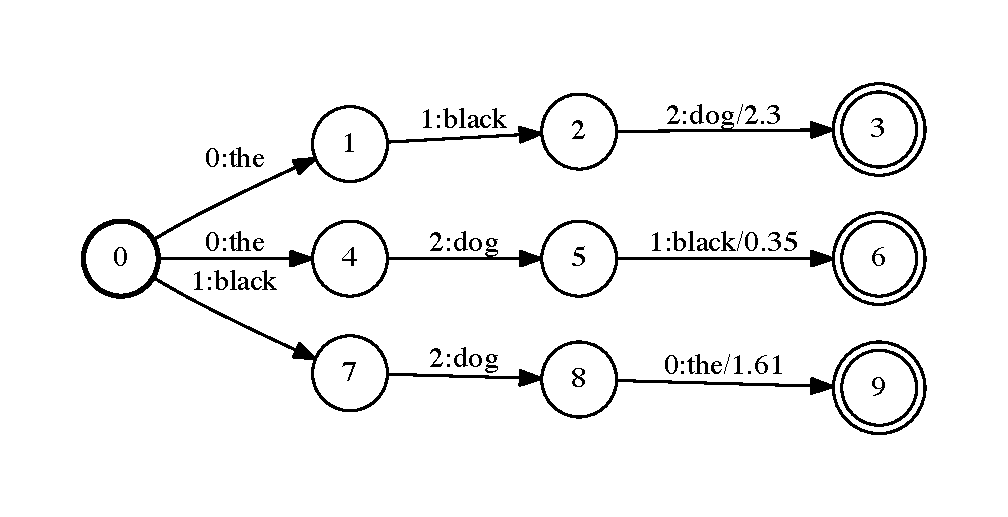
\includegraphics[scale=0.5]{permutations-list.pdf}
\caption{\label{fig:permutations}List of permutations as a non-deterministic transducer.}
\end{figure}


In order to discriminate alternative permutations, we will add a feature to our linear model. 
This feature is the negative log-probability of the permutation and the model parameter associated with it is called \texttt{LatticeCost}.
Table \ref{tab:task5} summarises the task. 

\begin{figure}[h]\centering
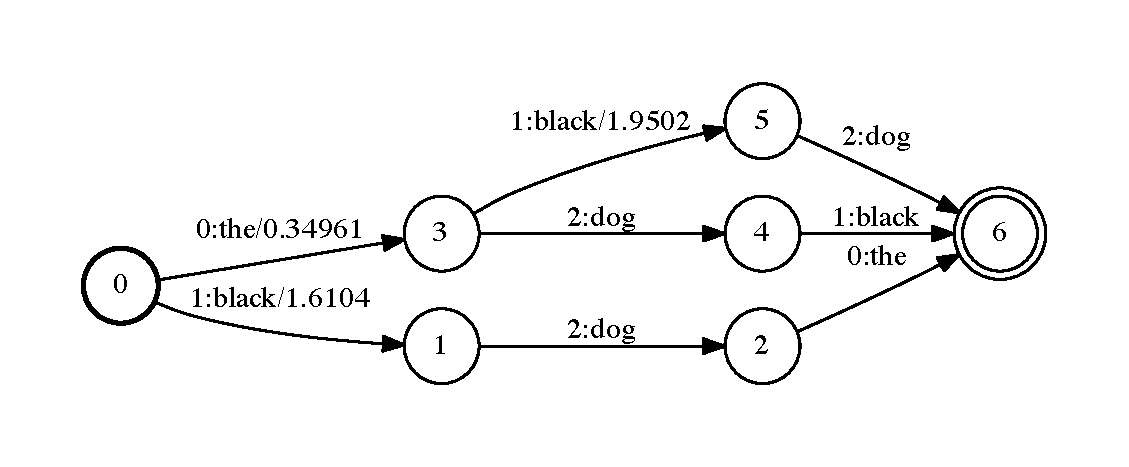
\includegraphics[scale=0.5]{permutations-lattice.pdf}
\caption{\label{fig:pi-det-min}Permutations packed in a deterministic transducer.}
\end{figure}

\begin{table}[h]\centering
\begin{tabular}{l p{12cm}}
\textsc{Task}   &  pack permutations into weighted lattices\\
\textsc{Input}  &  up to 100 permutations per source sentence \\
\textsc{Output} &  a permutation lattice per source sentence\\
\textsc{Submit} &  nothing to submit here\\  
\textsc{Report} & discuss the strategies for packing: e.g. determinisation and minimisation\\
\end{tabular}
\caption{\label{tab:task5}Task 5 summarised}
\end{table}


\subsection{Task 6: lattice translation}

A simple (though inefficient) way to translate a source sentence in non-monotone order would be to enumerate all alternative permutations and translate them individually.
Then, with some appropriate decision rule, we select the final translation.
Besides inefficient, some decision rules can only be defined in the combined space of translations.

Now that the permutations have been efficiently represented using transducers, translating these permutations is no different from translating a trivial linear finite-state transducer.
That is right, all it takes is a composition between the input lattice and the phrase-table transducer.
Figure \ref{fig:non-mono} illustrates the composition between the permutation lattice in Figure \ref{fig:permutations} and the phrase table in Figure \ref{fig:rules}.

\begin{figure}[h]\centering
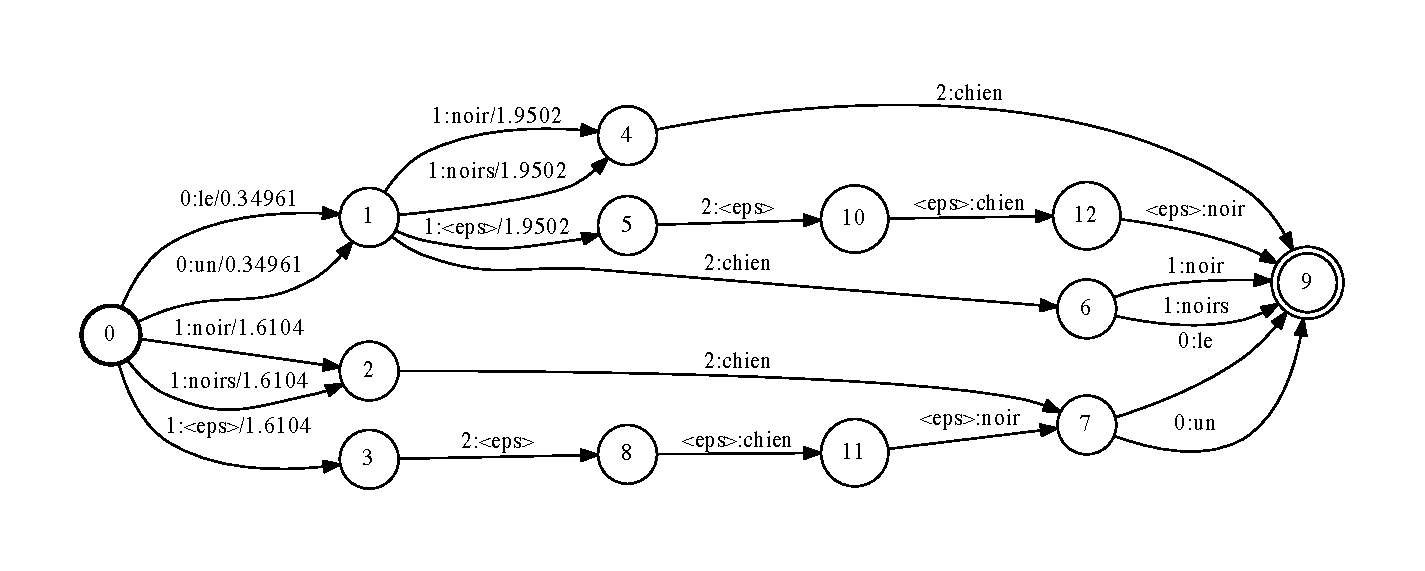
\includegraphics[scale=0.5]{lattice-nonmonotone.pdf}
\caption{\label{fig:non-mono}Translation derivations for permutations of the input.}
\end{figure}


Because we have changed the space of translations of our model (by including translations of permutations of the input), and because we have added a new feature to the linear combination (i.e. \texttt{LatticeCost}), it makes sense to re-estimate the parameters of the linear model.
You will not need to do it yourself,\footnote{But wait for project 3 ;)} as I have already provided you with \texttt{weights.lattice}.
You will need, however, to recompile your phrase tables so that they are weighted by the correct linear model.
Table \ref{tab:task6} summarises the task. 




\begin{table}[h]\centering
\begin{tabular}{l p{12cm}}
\textsc{Task}   &  translate permutation lattices\\
\textsc{Input}  &  one permutation lattice per sentence and a recompiled weighted transducer per phrase table\\
\textsc{Output} &  a weighted set of translation derivations per sentence\\
                &  100-best paths from each transducer \\
                & \emph{best-derivation} and \emph{best-translation} decision rules\\
\textsc{Submit} & \texttt{lattice.100best.}$n$: 100-best derivations from each transducer in text format with alignments\\
                & \texttt{lattice.der} and \texttt{lattice.trans} \\  
\textsc{Report} & BLEU score for each decision rule using references in \texttt{dev.ja}\\
\end{tabular}
\caption{\label{tab:task6}Task 6 summarised}
\end{table}




